
\chapter{Supervised Learning}

\section{Assessment}

The main axes of assessment are:
\begin{itemize}
    \item \inlinecode{Effectiveness}: how well the model performs on the test set.
    \item \inlinecode{Efficiency}: how much time and resources are needed to train the model (achieving the goal).
    \item \inlinecode{Interpretability}: how well the model can be understood by humans.
\end{itemize}

There are two purposes for assessment:
\begin{itemize}
    \item \textbf{Absolute Assessment:} does something meet the expectation with respect to a determined axis?
    \item \textbf{Comparison:} is one thing better than one other thing in terms of the determined axis? 
\end{itemize}

If the output of the assessment is a \inlinecode{quantity}, than a simple check for < or > is enough, so we want a number as output.

A \textbf{ML system} can be seen as a composite learning technique. It has two running modes: one in which it tunes itself and the other in which it makes decisions. The goals are:
\begin{itemize}
    \item \textbf{Training:} tune the model to minimize the error on the training set (tuning properly).
    \item \textbf{Testing:} evaluate the model on the test set (making good decisions).
\end{itemize}

The SLT has then this two goals, while a \textbf{model} has the only goal to make good decision when used in an $f'_{predict}$.

To measure the \textbf{effectiveness} of a model and to have a number as output, we need to compare our system with the real system that generated the data (assuming there is one).

\begin{figure}[H]
    \centering
    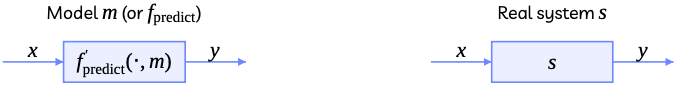
\includegraphics[width=0.7\textwidth]{assets/fig3.png}
    \caption{Model vs Real System}
\end{figure}

\definitionblock[Model vs Real System]{
    \begin{itemize}
        \item Collect examples of \textbf{s} behavior
        \item Feed \textbf{m} with examples 
        \item Compare responses of \textbf{s} and \textbf{m}
    \end{itemize}
    \textbf{Effectiveness:} to which degree the comparison step measures if m behaves like s.
}

\warningblock[$f_{collect}$]{
    The data collection is really important, since:
    \begin{itemize}
        \item small n $\to$ \textbf{poor} effectiveness, \textbf{great} efficiency
        \item large n $\to$ \textbf{good} effectiveness, \textbf{poor} efficiency
    \end{itemize}
    (effectiveness = accuracy, efficiency = resources)

    and also:
    \begin{itemize}
        \item poor coverage $\to$ \textbf{poor} effectiveness
        \item good coverage $\to$ \textbf{good} effectiveness
    \end{itemize}
    where coverage = how well the data represents the real system.
}

\begin{center}
    \begin{figure}[H]
        \centering
        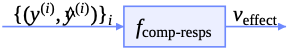
\includegraphics[width=0.5\textwidth]{assets/fig4.png}
        \caption{Comparing the responses}
    \end{figure}
\end{center}

where ${(y^{(i)}, \hat{y^{(i)}})}_i \in P^* (Y^2)$ is a multiset of pairs of y.

\exampleblock[Performance Indexes]{
    \textbf{Classification:}
    \begin{itemize}
        \item all types $\to$ error, accuracy 
        \item binary $\to$ EER, AUC, FPR, FNR and variants
        \item multi-class $\to$ weighted accuracy
    \end{itemize}
    \textbf{Regression:}
    \begin{itemize}
        \item MSE, MAE, R2
    \end{itemize}
}

\subsection{Classification}

In \inlinecode{Classification} Y is a finite set with no ordering.

The \textbf{Classification Error} is then 
\begin{center}
    $f_{err}({y^{(i)}, \hat{y^{(i)}}}) = \frac{1}{n}\sum_{i=1}^{i=n}\textbf{1}(y^{(i)} \neq \hat{y^{(i)}})$
\end{center}

where \textbf{1(b)} is the indicator function and takes value 1 when (in this case) the prediction is wrong.

The \textbf{Classification Accuracy} is instead:
\begin{center}
    $f_{acc}({y^{(i)}, \hat{y^{(i)}}}) = \frac{1}{n}\sum_{i=1}^{i=n}\textbf{1}(y^{(i)} = \hat{y^{(i)}})$
\end{center}

\textbf{Reminder:} $f_{acc} = 1 - f_{err}$

Extreme cases for accuracy (and errors) are:
\begin{itemize}
    \item m is s: \textbf{perfect model}
    \item m is random: does not model any dependence
\end{itemize}

\exampleblock[Random Classifier - Lower Bound]{
    $f_{random}(x) = y_i$ with $i ~ U({1, \dots, |Y|})$     just pick random uniformly
}
\exampleblock[Dummy Classifier - Better Lower Bound]{
    $f_{dummy}(x) = argmax \frac{1}{n} \sum_{i=1}^{i=n}\textbf{1}(y = y^{(i)})$     just pick the category with more example always
}
\exampleblock[Perfect Classifier - Upper Bound]{
    $f_{perfect}(x)= s(x)$
}
But the world is not deterministic, so a Bayes (stochastic) classifier may be better:
\exampleblock[Bayes Classifier - Better Upper Bound]{
    $f_{Bayes}(x) = argmax Pr(s(x) = y | x)$
}

\subsection{Binary Classification}

The main problem here are the \inlinecode{skewed datasets}, meaning the datasets with more example of a category than the other (we are considering only two categories here).

\definitionblock[FPR - False Positive Rate]{
    It is the rate of \textbf{negatives} that are wrongly classified as positives

    $FPR = \frac{FP}{N}$
}
\definitionblock[FNR - False Negative Rate]{
    It is the rate of positives that are wrongly classified as negatives.
    $FNR = \frac{FN}{P}$
}
Where
\begin{itemize}
    \item FP = False Positives 
    \item FN = False Negatives 
    \item P = Total positives 
    \item N = Total Negatives 
\end{itemize}

\begin{center}
    \begin{figure}[H]
        \centering
        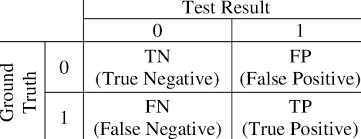
\includegraphics[width=0.5\textwidth]{assets/fig5.png}
        \caption{Confusion Matrix}
    \end{figure}
\end{center}

\inlinecode{TPR:} True Positive Rate = 1 - FNR

\inlinecode{FPR:} False Positive Rate = 1 - TNR

\inlinecode{Err:} Error Rate = $\frac{FP + FN}{P + N}$

\inlinecode{Acc:} Accuracy = $\frac{TP + TN}{P + N}$

\definitionblock[Balanced Data]{
    In classification, a dataset is \textbf{balanced} with respect to the response variable y, if the frequency of each value of y is roughly the same.
}

\inlinecode{Precision:} $\frac{TP}{TP + FP}$

\inlinecode{Recall:} $\frac{TP}{TP + FN}$

\inlinecode{F1:} $2 \cdot \frac{Precision \cdot Recall}{Precision + Recall}$

\inlinecode{Sensitivity:} $\frac{TP}{TP + FN} = TPR$

\inlinecode{Specificity:} $\frac{TN}{TN + FP} = TNR$

\inlinecode{Type I error:} False Positive Rate = FPR 

\inlinecode{Type II error:} False Negative Rate = FNR

\warningblock[Cost of the error]{
    Once $f_{predict}$ outputs a y, some action is taken, and if the action is wrong, there is some cost to be paid wrt the correct action.

    $c = c_{FP} \times FPR \times N + c_{FN} \times FNR \times P$

    If one knows the costs and N,P, it is possible to compute the overall cost and find a good trade-off for FPR and FNR.
}

Given a model, we can "tune" it to prefer avoiding FPs rather than FNs, just by modifying the threshold that is used to determine the choice to be made wrt the category.
Many learning techniques compute a probability distribution over Y before returning one y, and in the case of Binary Classification the threshold is 0.5. 

\begin{center}
    \begin{figure}[H]
        \centering
        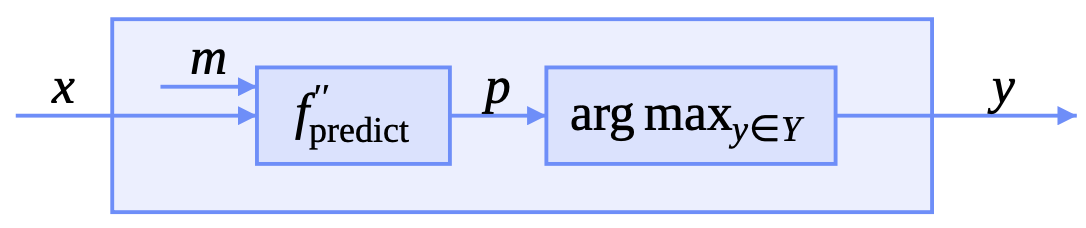
\includegraphics[width=0.5\textwidth]{assets/fig6.png}
        \caption{Threshold}
    \end{figure}
\end{center}
\newpage
So, by varying the threshold we can change FPR and FNR:
\begin{itemize}
    \item the greater the threshold, the lower FPR and the greater FNR
    \item the lower the threshold, the greater FPR and the lower FNR
\end{itemize}

\begin{center}
    \begin{figure}[H]
        \centering
        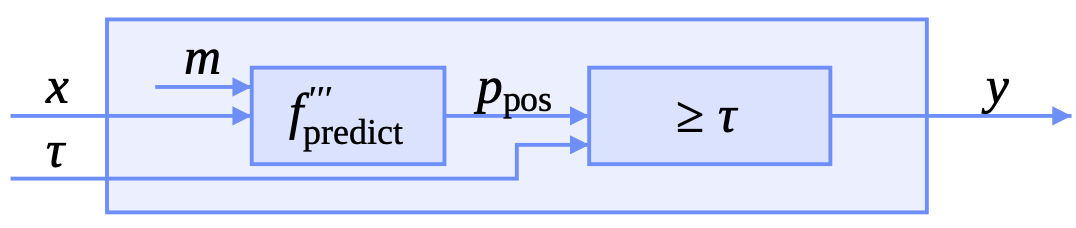
\includegraphics[width=0.5\textwidth]{assets/fig7.png}
        \caption{Threshold}
    \end{figure}
\end{center}

\definitionblock[ROC Curve (Receiver Operating Characteristic)]{
    The ROC curve is a graphical representation of the trade-off between the True Positive Rate (TPR) and the False Positive Rate (FPR) for every possible threshold.
}

\begin{center}
    \begin{figure}[H]
        \centering
        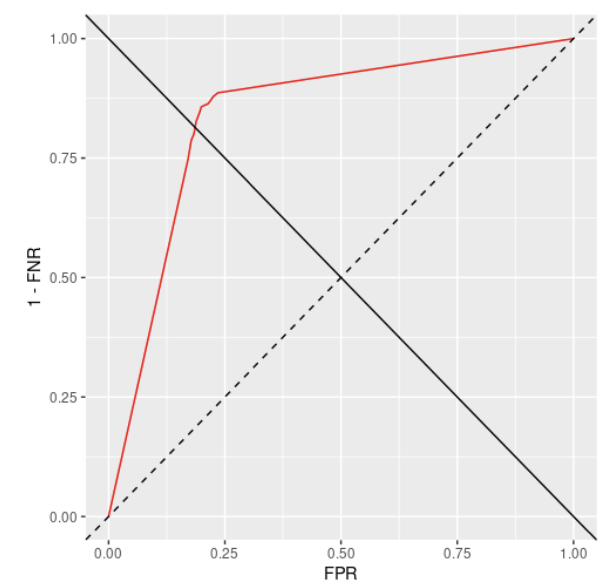
\includegraphics[width=0.5\textwidth]{assets/fig8.png}
        \caption{ROC Curve}
    \end{figure}
\end{center}

The dotted line represents the random classifier, while the closer the curve is to the top-left corner, the better the classifier is.

How to choose the threshold? Take different values and compute the ROC curve, then choose the one that is closer to the top-left corner. To do this, the best way is to take the \textbf{midpoints} of the sorted probabilities.

\newpage 

\subsection{Multiclass Classification and Regression}

Here we use the concept of \textbf{weighted accuracy}, which is 
    
    $f_{acc} = \frac{1}{|Y|}\sum_{y \in Y}^{}Acc_y$

\begin{figure}[H]
    \centering
    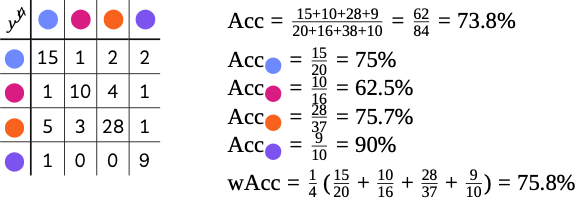
\includegraphics[width=0.5\textwidth]{assets/fig9.png}
    \caption{Multiclass Confusion Matrix}
\end{figure}

Moreover, the error there is different from the classification one: here we measure the \inlinecode{distance} from the real value.

\begin{itemize}
    \item \inlinecode{MAE:} Mean Absolute Error = $\frac{1}{n}\sum_{i=1}^{i=n}|y^{(i)} - \hat{y^{(i)}}|$
    \item \inlinecode{MSE:} Mean Squared Error = $\frac{1}{n}\sum_{i=1}^{i=n}(y^{(i)} - \hat{y^{(i)}})^2$   
    \item \inlinecode{RMSE:} Root Mean Squared Error = $\sqrt{MSE}$
    \item \inlinecode{MAPE:} Mean Absolute Percentage Error = $\frac{1}{n}\sum_{i=1}^{i=n}\frac{|y^{(i)} - \hat{y^{(i)}}|}{y^{(i)}}$
\end{itemize}

\subsection{Assessing Learning Techniques}
\begin{itemize}
    \item an \textbf{effective} learning technique is a pair of $f'_{learn}$, $f'_{predict}$ that learns a good model $m$
    \item a good \textbf{model} is one that has the same behavior of the real system $s$
\end{itemize}

We, then, want to measure the effectiveness of the learning techniques (learning and prediction).
To do so, we need to divide the dataset, since we want to see if the $f'_{predict}$ generalises well.

\definitionblock[Static Train/Test Division]{
    \begin{itemize}
        \item \textbf{Effectiveness:} generalization is assessed, but there is no robustness wrt D division 
        \item \textbf{Efficiency:} learning is executed only once 
    \end{itemize}
    $D_{test}$ is the unseen data and we treat is as said even if it has been collected at once with $D_{train}$.
}

\definitionblock[Repeated random train/test division]{
    \begin{itemize}
        \item \textbf{Effectiveness:} generalization is assessed, and there is robustness wrt D division 
        \item \textbf{Efficiency:} learning is executed multiple times \propto k
    \end{itemize}
}

\definitionblock[Cross-Validation]{
    \begin{itemize}
        \item \textbf{Effectiveness:} generalization is assessed, and there is robustness wrt D division 
        \item \textbf{Efficiency:} learning is executed multiple times \propto k
    \end{itemize}
}

\definitionblock[Leave-One-Out]{
    \begin{itemize}
        \item \textbf{Effectiveness:} generalization is assessed, and there is robustness wrt D division 
        \item \textbf{Efficiency:} learning is executed multiple times \propto n 
    \end{itemize}
    This is the worst case for efficiency, since we repeat the learning phase n times.
}

\begin{center}
    \begin{figure}[H]
        \centering
        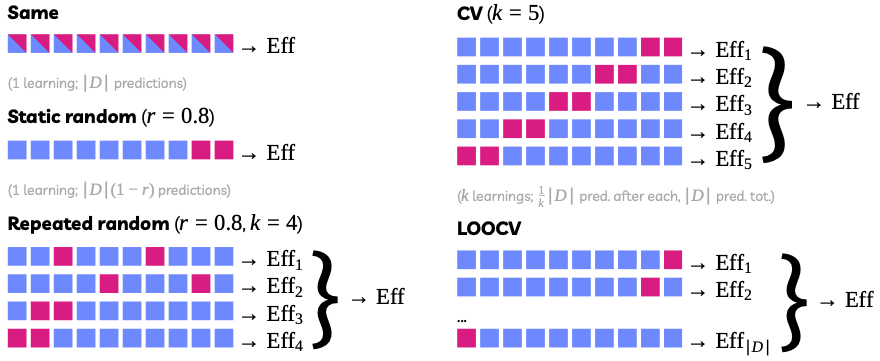
\includegraphics[width=0.8\textwidth]{assets/fig10.png}
        \caption{Train/Test Division Methods}
    \end{figure}
\end{center}

For comparison btw learning techniques, we can use the mean and standard deviation of the performance indexes obtained with the previous division methods. \textbf{Boxplots} are useful in this case.

\section{Tree-based Learning Techniques}

\subsection{Decision Trees}

A \textbf{Decision Tree} is a tree where each node is a decision on the value of a feature, and each branch is a possible value of the feature. The leaves are the categories. It can be understood in simpler terms by considering a basic \inlinecode{if-then-else} nested structure.

\begin{center}
    \begin{figure}[H]
        \centering
        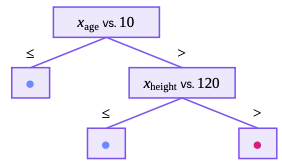
\includegraphics[width=0.5\textwidth]{assets/fig11.png}
        \caption{Decision Tree example}
    \end{figure}
\end{center}

This is a binary tree, but it can be n-ary as well. The tree is built by recursively splitting the dataset into subsets, and the splitting is done by selecting the feature that best splits the dataset into the purest subsets. The purity is measured by the \inlinecode{Gini Index} or the \inlinecode{Entropy}, usually.

One can also represent the tree in a compact way:
\begin{center}
    $t = [l, t', t'']$
\end{center}

where $l \in L$ is the \textbf{label} and $t', t'' \in T_L \cup \{\emptyset\}$ are the left and right children.

Also, each \textbf{non-terminal} node is a pair ($j, \tau$), where $j \in \{1, \dots, p\}$ is the index of the independent variable and $\tau \in R$ is the threshold for comparison.

The above figure is then represented as:

\begin{center}
    \begin{figure}[H]
        \centering
        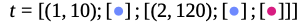
\includegraphics[width=0.5\textwidth]{assets/fig12.png}
        \caption{Compact representation of the Decision Tree}
    \end{figure}
\end{center}
